\documentclass[main.tex]{subfiles}
\begin{document}
  \section{Evaluating the Model}
      
      The model has been assessed by comparing it to data from real matches. \\
      In this process a small subset of data was dedicated as the "training" set, and used to adjust the model and inform modelling decisions. The remaining data was designated the "test" set that was used upon development completion to evaluate the model.
      
      \subsection{Data Aquision}
        
        Data was taken from the FIVB Men's World Championship \cite{dataGames}, while focusing on Poland's team, by noting down relevant data in excel, based on the defined model. This was done early on in development, as mentioned previously. Specifically the data included the game's score, the coordinates the setter came in contact with the ball, the position the setter decided to set to, the success of the attack and mistakes that were made, among others.
        \\\\
        While this was done early in the development, it quickly became clear that a number of parameters, like mistakes in passing and sets from very difficult positions, were beyond the scope of the model. These phenomena involve a fair degree of rather unpredictable factors and would uunnecessarily complicate the model.
        \\\\
        Furthermore, from the impressions these games left it was possible to form design decisions, in particular those that fine tuned the model. For example, position 3 stands out by being extremely viable when the setter is close, but always being a bad choice when the setter is even slightly further away. This is different from other positions, that are generally still viable from slightly further away, and has to do with its central position, as the opponent can gang up on this position easily and quickly, unlike in other positions.\\
        
      \subsection{Analysis}
        
        The single most powerful description of the model's accuracy, quite obviously, is its ability to find the best position to set to. This should be the position that is scored highest by the model, and ideally also the position the real world setter decides to set to.\\
        As there is real world data on what the setter would have considered the second best choice at the time, this is largely the only parameter available to asses the accuracy of the model.
        \\\\
        For each prediction the model records whether the real setter's choice was scored highest (i.e. 1), second highest (i.e. 2) etc. This was dubbed the choice-rank-score. \\
        After development completed the model was tuned by adjusting \(ease_{attack}\) weights, among others, to maximise the choice-rank-score. \Cref{fig:training} shows the model's performance after tuning. \\
        Subsequently \Cref{fig:test} shows the chooice-rank-score on the larger test set. It would appear that the larger the data set the more clearly the choice-rank-score follows some linear curve.
        \\\\
        \begin{figure}[h!]
          \begin{subfigure}{0.5\linewidth}
            \centering
            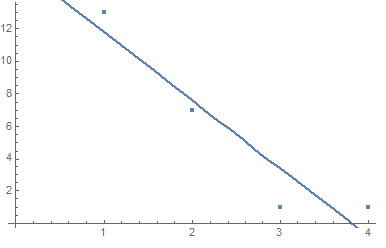
\includegraphics[width=0.80\linewidth]{figures/trainingGraph}
            \caption{Model Performance on Training Data}
            \label{fig:training}
          \end{subfigure}
          \begin{subfigure}{0.5\linewidth}
            \centering
            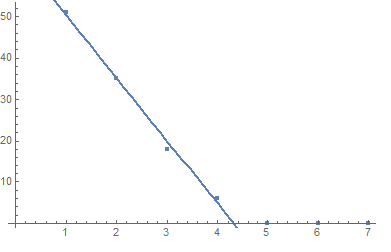
\includegraphics[width=0.80\linewidth]{figures/testGraph}
            \caption{Model Performance on Test Data}
            \label{fig:test}
          \end{subfigure}
          \caption{Model Performance on Training and Test Data Sets. \\
            Trendlines show that the model is representative of the choices made by a real setter. Null Hypotheses were rejected at the 5\% margin for the training and at the 1\% margin for the test set. \\
            Note that regression was performed on the valid choices, taking into account that there are at least two invalid positions that cannot be chosen at any time.
            }
          \label{fig:analysis}
        \end{figure}
        
        Clearly, the model is capable of rather accurately predicting the probability of the setter to set to a particular position.
        
      \subsection{Drawbacks}
        
        The most evident drawback of the model is that there are a significant number of sets that are scored only second or even third. These are mostly attributed to the fact that setters should not be too predictable, as their opponents would be able to adapt better otherwise. 
        \\\\
        Another issue with this analysis is the focus on only one real world setter. It is possible that it is, in a sense, "over-trained" on just this setter and will perform worse with other setters.
        \\\\Finally, in future iterations the model could begin to take the opposing team into account. Likely this would require keeping track of all players and their likely positions at the time that the ball would contact the player, slightly after the set happened. \\
       However, beyond the difficulty of incorporating this into the model, it would be even more difficult to acquire data for this purpose. It is very well possible that the current method of data acquisition would prove inadequate in this scenario and more automated methods would have to be explored.
      

\end{document}